% This file is part of the Open Source project 'proTironeComputatri'
% (c) 2025 Karsten Reincke (https://github.com/pro-tirone-computatri/protico.ltx)
% It is distributed under the terms of the creative commons license
% CC-BY-4.0 (= https://creativecommons.org/licenses/by/4.0/)

\selectlanguage{ngerman}

{
\usebackgroundtemplate{\includegraphics[width=\paperwidth]{\imgLf/woman-considering-1080572-pxh.png}}
\begin{frame}  
  \frametitle{LF09:00:Curriculum}

  \vspace{4cm}
  \begin{flushright}
    \textcolor{blue}{Wer bestimmt eigentlich, \\
    was \textit{Fachinformatikerinnen} \\
    für die AP1 und AP2 \\
    lernen müssen?}
  \end{flushright}
\end{frame}
}

\begin{frame}  
  \frametitle{LF09:00:Curriculum:Entscheiderinnen}
  \begin{center}
  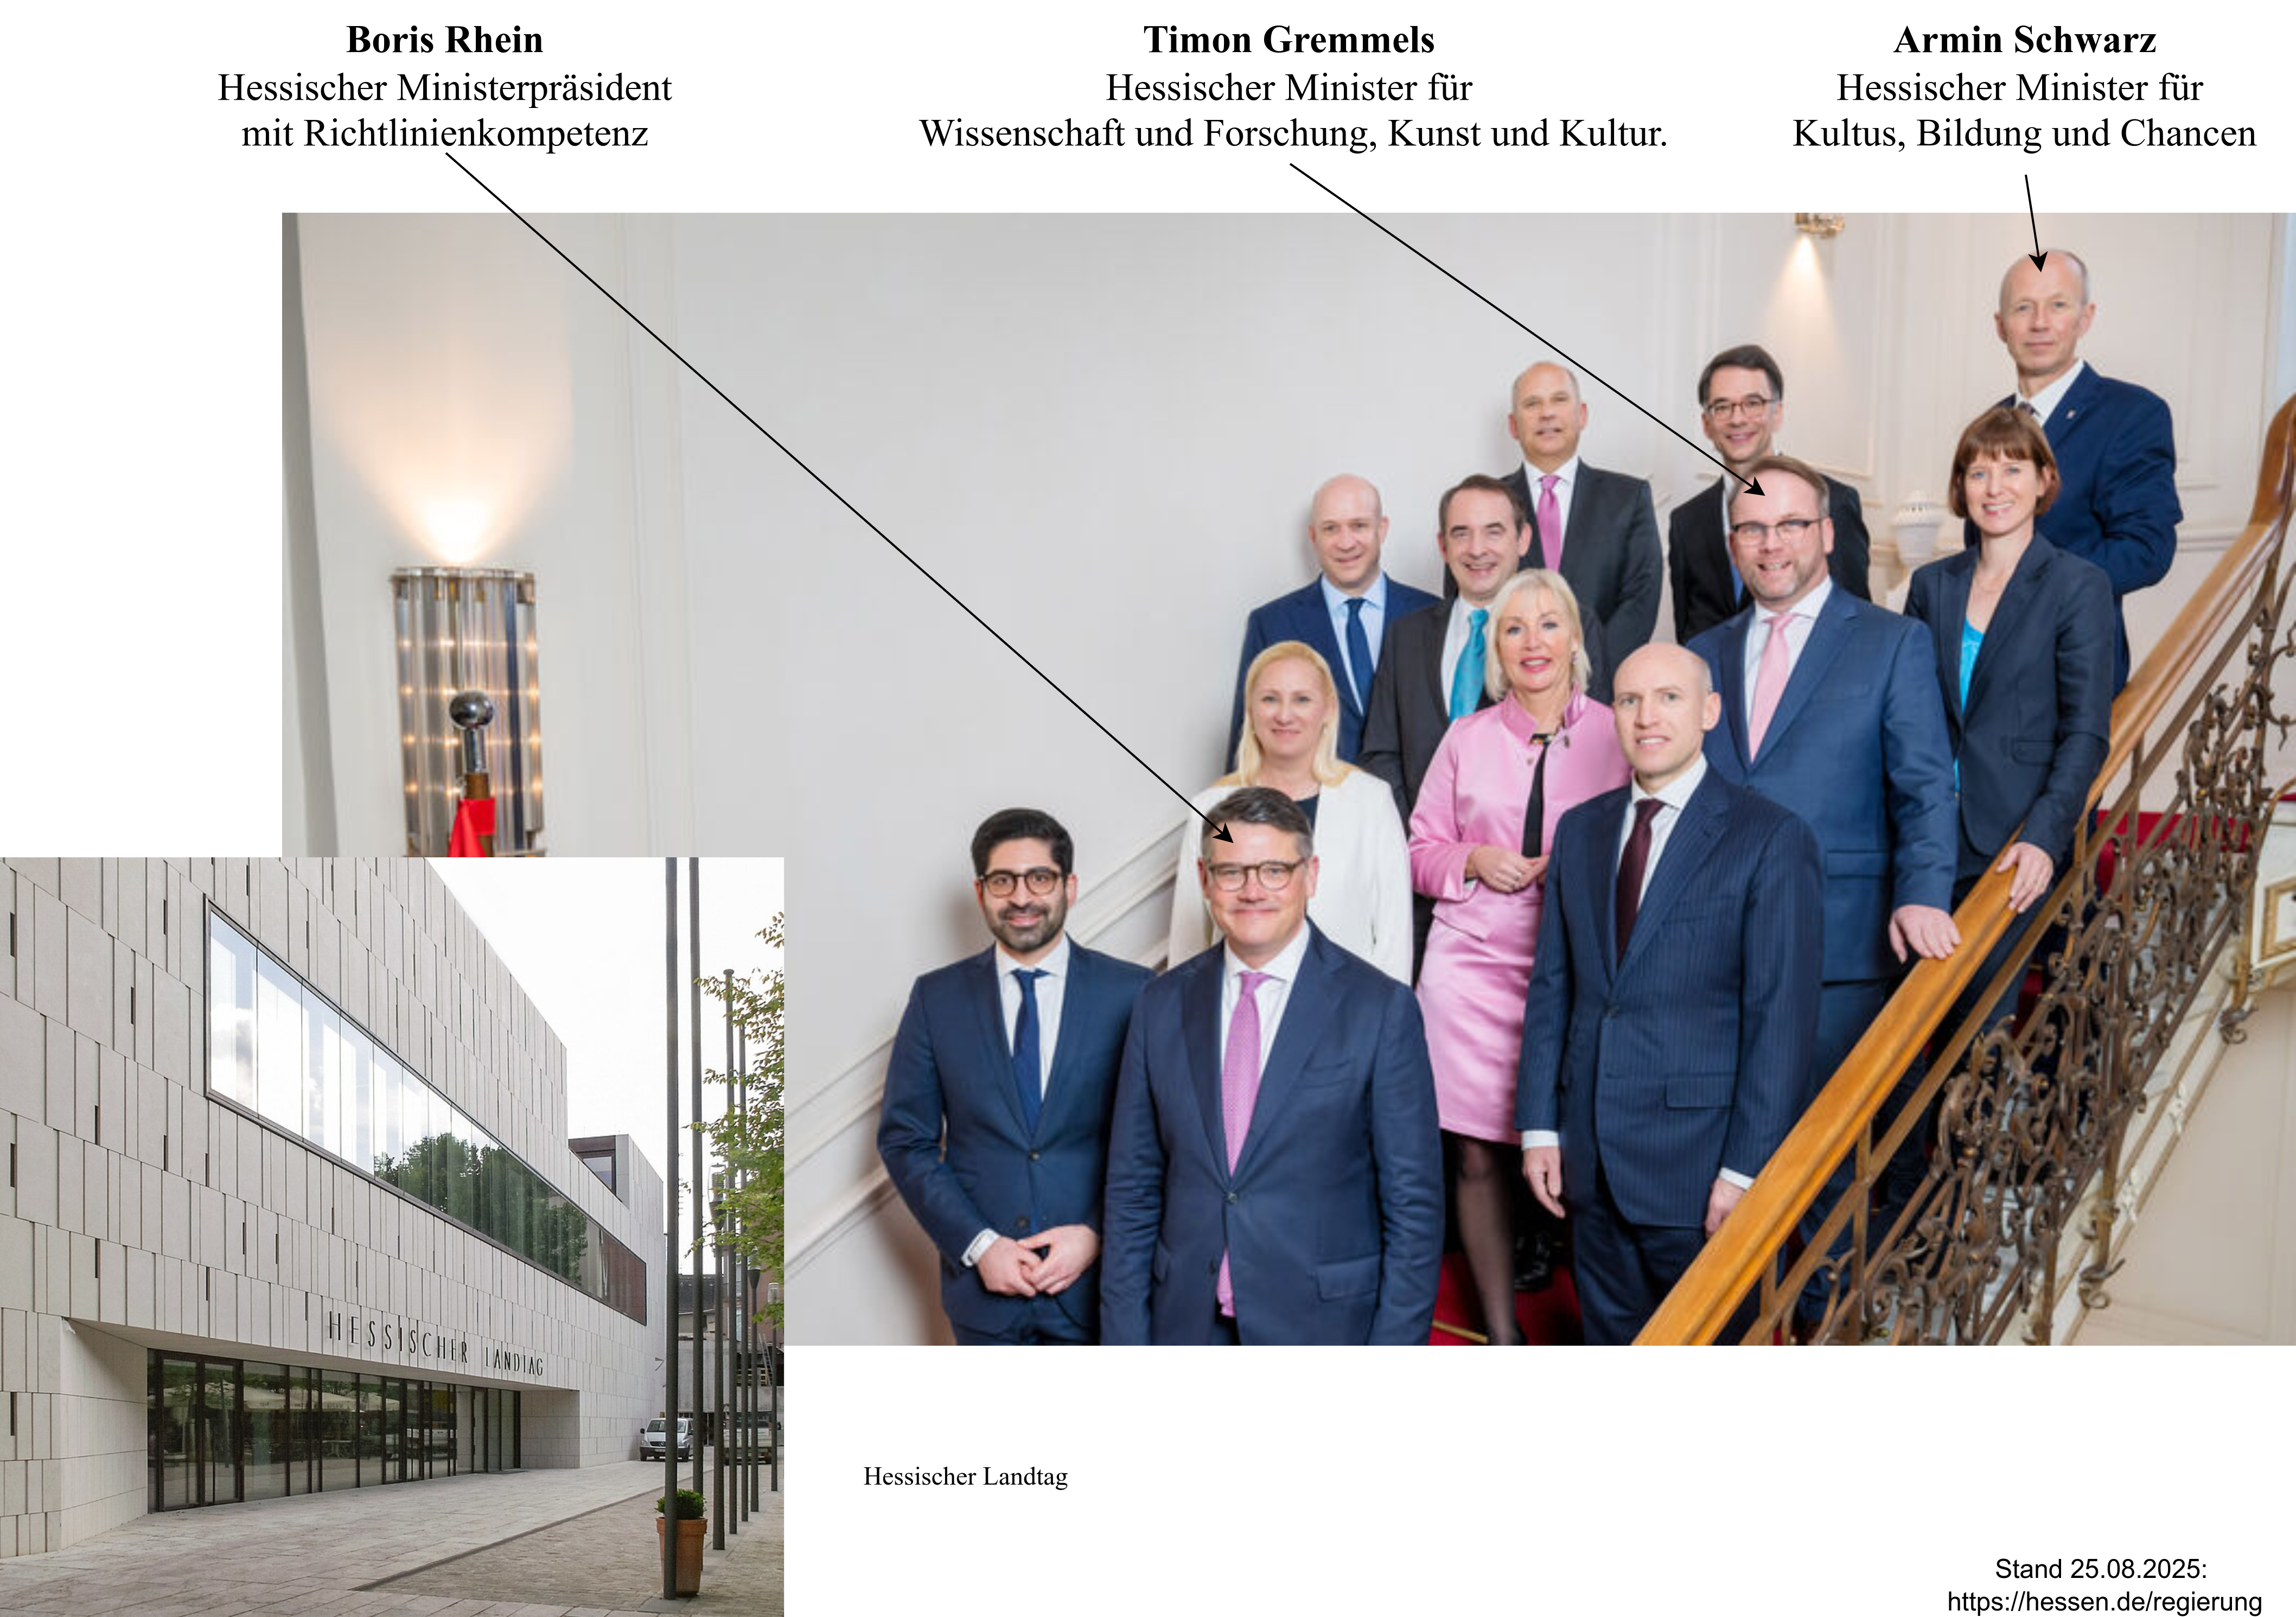
\includegraphics[width=10cm]{\imgGl/hessen-regierung.png}
  \end{center}
\end{frame}

{
\usebackgroundtemplate{\includegraphics[width=\paperwidth]{\imgLf/smartphone-4669-pxh.png}}
\begin{frame}  
  \frametitle{LF09:00:Curriculum:Entscheidungsbeispiel}

  \vspace{6cm}
  \begin{flushright}
    \textcolor{white}{Hessens neue Handyregelung!}
  \end{flushright}
\end{frame}
}

{
\usebackgroundtemplate{\includegraphics[width=\paperwidth]{\imgLf/fragmenting-759708-pxh.png}}
\begin{frame}  
  \frametitle{LF09:00:Curriculum:Fragmentierung}

  \vspace{7cm}
  \begin{flushright}
    \textcolor{magenta}{Jedes Land für sich?}
  \end{flushright}
\end{frame}
}

\begin{frame}
  \frametitle{LF09:00:Curriculum:supraförderal}
  \begin{figure}
    \includegraphics[width=10cm]{\imgGl/kmk-logo.png}
  \end{figure}
\end{frame}

\begin{frame}
  \frametitle{LF09:00:Curriculum:supranational}
  \begin{figure}
    \includegraphics[height=7cm]{\imgGl/kmk-rfdr.png}
  \end{figure}
\end{frame}

\begin{frame}
  \frametitle{LF09:00:Curriculum:Gendern}
  \begin{figure}
    \includegraphics[width=10cm]{\imgGl/gendern-934569-pxh.png}
  \end{figure}
\end{frame}


\begin{frame}
  \frametitle{LF09:00:Curriculum:KMK-Entscheidung}
  \begin{figure}
    \includegraphics[height=7cm]{\imgGl/kmk-rlp-fi-head.png}
  \end{figure}
\end{frame}

\begin{frame}
  \frametitle{LF09:00:Curriculum:Lernfelder}
  \begin{figure}
    \includegraphics[height=7cm]{\imgGl/kmk-rlp-lf-structure.png}
  \end{figure}
\end{frame}


\begin{frame}
  \frametitle{LF09:00:Curriculum:Prüfungskataloge}
  \begin{columns}
    \column{0.7\textwidth}
      Prüfungskataloge
      \begin{itemize}
        \item werden durch die \textit{Zentralstelle für Prüfungsaufgaben} der \textit{IHK} erstellt
        \item leiten aus dem Rahmenlehrplan abfragbare Themen ab
        \item sind in 2024 neu formuliert worden
        \item werden vom U-Form-Verlag veröffentlicht
        \item stellen klar, dass LF09-Inhalte in die AP2 gehören, nicht in die AP1\footnote{\tiny{erlauben aber, dass LF03 Themen (auch) in AP2 vorkommen}}.
      \end{itemize}

    \column{0.3\textwidth}
      \includegraphics[height=3.6cm]{\imgGl/pruefkatalog-ip.png}
      
      \includegraphics[height=3.6cm]{\imgGl/pruefkatalog-iv.png}
  \end{columns}
\end{frame}

